\documentclass[runningheads,a4paper,draft]{IEEEtran} % TODO remove draft mode
\usepackage{booktabs}
\usepackage[hidelinks]{hyperref}
\usepackage{pgfplots}
\usepgfplotslibrary{fillbetween}
\usetikzlibrary{patterns}
\usepackage{multicol} % For 2 columned bullet point list
\usepackage{caption} % To improve laf of captions (also imported by subcaption)
\usepackage{mathtools} %For = aligned equations
\usepackage[final]{listings} %For microbenchmark code listing TODO: final prevents draft mode hiding listings. Remove for publication.
\usepackage{subcaption} % For putting figures 2-up
\usepackage[T1]{fontenc} % For literal \{ and \} in author emails
\pgfplotsset{compat=1.12}

\newtheorem{definition}{Definition} %Hack to allow definition in IEEE
\title{POSE: A New Technique to Guide Energy Aware Code Optimisation}

\newcommand{\DRAFT}[1]{•}
\renewcommand*{\sectionautorefname}{Section} % make sec: autorefs capitalized.

\date{}
%COMMANDS

\newcommand{\todo}[1]{•}

\ifdefined\DRAFT
	\usepackage{color} %Used for colored text (TODO)
	\renewcommand{\todo}[1]{{\color{red} TODO: {#1}}} % comment me out for prod  
\fi 

\definecolor{printred}{RGB}{215,25,28}
\definecolor{printorange}{RGB}{253,174,97}
\definecolor{printyellow}{RGB}{255,255,191}
\definecolor{printgreen}{RGB}{145,180,130}
\definecolor{printblue}{RGB}{43,131,186}
\definecolor{printlilac}{RGB}{178,171,210}

\pgfplotsset{
    legend image with text/.style={
        legend image code/.code={%
            \node[anchor=center] at (0.3cm,0cm) {#1};
        }
    },
}
\newcommand{\legendline}[1]{%
  \raisebox{2pt}{\tikz{\draw[#1](0,0) -- (4.5mm,0);}}%
}

\begin{document}
  \maketitle
  \begin{abstract}
Performance engineers are beginning to explore software-level optimisation as a means to reduce the energy consumed when running their codes.
This paper presents POSE, a mathematical and visual model of the relationship between runtime and power consumption for a particular code and architecture.
POSE allows developers to assess how much improvement can be expected from power optimisations and hence whether they are worth pursuing.

We demonstrate POSE by studying the power optimisation characteristics of codes from the Mantevo and Rodinia benchmark suites.
We show that LavaMD has the most scope for CPU power optimisation out of these codes, with the potential to improve Energy Delay Squared Product by up to 30.59\%.
Conversely, MiniMD offers the least scope with improvements to the same metric limited to 7.60\%.
We also consider the effect frequency scaling has on the scope for power optimisation.
\end{abstract}

  \section{Introduction}
Advances in processor design have delivered improvements in CPU performance for decades. As physical limits are reached, however, refinements to the same basic technologies are beginning to show diminishing returns \cite{esmaeilzadeh:2011aa}. One side-effect of this is an unsustainable rise in system power use, which the US Department of Energy has identified as a primary constraint for exascale systems \cite{shalf:2011aa}.

Hardware manufacturers are increasingly prioritising energy efficiency in processor designs~\cite{kurd:2014aa}. 
Research suggests that software modifications will be required to fully exploit the resulting improvements in modern processors~\cite{shao:2013aa}.

In this paper we present the Power Optimised Software Envelope (POSE).
POSE is a visual model which provides insights into the energy consumption characteristics of a code.
Our work helps performance engineers understand whether power or runtime optimisation is the best strategy for improving the energy efficiency of their codes.

\medskip \noindent
The contributions made in this work are:
\begin{itemize}
  \item We introduce the POSE model, providing derivations for its constituent boundaries and an overview of the insights it offers.
  \item We show how POSE, which is a general technique, can be targeted to specific platforms and use-cases. 
        Specifically, we investigate the trade-offs between runtime and CPU power consumption.
  \item We employ POSE in a comparative study of codes from the Mantevo and Rodinia application suites. 
        We assess the potential benefits of power optimisation for each code, showing that LavaMD offers the most scope for power optimisation while MiniMD offers the least.
        We also investigate how opportunities for power optimisation vary in response to frequency scaling for these two codes.
\end{itemize}

The remainder of this paper is structured as follows: \autoref{sec:related} outlines different approaches to performance modelling and explains where POSE fits in this landscape.
\autoref{sec:metrics} provides a summary of key concepts and metrics.
\autoref{sec:pose} details the construction of POSE and describes the various insights it provides.
We demonstrate our model in \autoref{sec:investigation} by using it to study the CPU power optimisation opportunities presented by a range of proxy applications. 
We end with conclusions and future work in \autoref{sec:conclusion}.

  \section{Related Work}
\label{sec:related}
Performance modelling techniques enable the rapid exploration of large hardware and software design spaces.
This section describes various approaches to performance modelling and explains how POSE fits into this area.
\autoref{tab:approaches} divides the performance modelling ecosystem into categories based on model domain and granularity and provides examples for each.

\begin{table}
  \centering
  \caption{Performance Model Classifications}
  \setlength{\tabcolsep}{10pt}
  \begin{tabular}{lll}
  \toprule
    & \multicolumn{2}{l}{Domain}\\ \cmidrule(){2-3}
  Model Type  & Runtime & Energy \\
    \midrule
  Simulation & SST~\cite{rodrigues:2011aa} & McPAT~\cite{li:2009aa}  \\
  Analytical & Bunt~\cite{bunt:2013aa} & Karkhanis~\cite{karkhanis:2007aa} \\
  Heuristic & Roofline~\cite{williams:2009aa} & \textbf{POSE} \\
  \bottomrule
  \end{tabular}
  \label{tab:approaches}
\end{table}

\subsubsection{Simulators:} 
Tools like SST~\cite{rodrigues:2011aa} and McPAT~\cite{li:2009aa} gather data while executing a simplified representation of the original code.
These approaches can be extremely insightful, however constructing and validating representative simulations is often challenging.
They also tend to be expensive to run, sometimes even more so than the original code.

\subsubsection{Analytical Models:} This approach distils the structure and performance of a program into parameterised expressions.
Examples of this technique are found in the work of Bunt~et~al.~\cite{bunt:2013aa} and Karkhanis~et~al.~\cite{karkhanis:2007aa}.
Analytical models produce results more quickly than simulations, making them particularly useful when performing parameter sweeps.
Ensuring the model is expressive enough to capture all possible program behaviours is the biggest obstacle to this approach as it requires a deep understanding of the target application.

\subsubsection{Heuristic Models:}
This is the most abstract category of performance models and the one in which our work belongs.
Rather than attempting to faithfully represent an entire system, heuristic models provide a simplified analogy which helps developers reason about particular properties of a code.
Ease of construction and the clarity of their insights mean heuristic models are well suited to guiding the early stages of optimisation.

A popular example of this class is the Roofline model~\cite{williams:2009aa}.
Roofline frames application performance in terms of its operational intensity and two system bottlenecks; off-chip memory bandwidth and floating point performance.
This simplification limits Roofline's use as a predictive model but it also means a developer can easily isolate the limiting factor of code performance and target their optimisation efforts accordingly.

The POSE heuristic serves as a preliminary `first cut' modelling technique intended to guide energy-aware optimisation efforts.
Our model provides an asymptotic analysis of the scope for optimisation in the power and runtime domains, allowing performance engineers to focus their efforts wherever they will be most beneficial.
POSE also takes after the Roofline model in that its insights can be presented in an intuitive graphical format.

  \section{Optimisation Metrics}
\label{sec:metrics}
\noindent
Energy is the integral of power consumed over time, or simply $E = \bar{P}t$.
As such, reducing the energy consumed by a code can be achieved either through shortening its runtime ($t$) with conventional program optimisations or reducing the average power consumption ($\bar{P}$) with power optimisations.
The POSE heuristic enables performance engineers to compare the potential benefits of each approach and focus their efforts on whichever offers the greatest rewards.

Energy to solution is a reasonable metric when energy consumption is of paramount importance.
This metric leaves open the possibility of significant loss of runtime performance however, limiting its usefulness in time-sensitive domains.
Metrics combining both runtime and energy costs have been developed to address this issue. 
The simplest of these is the Energy Delay Product (EDP) metric \cite{gonzales:1996aa}, which is defined as follows:
\begin{align}
  EDP &= Energy \times Runtime \nonumber \\
      &= E \times t \nonumber \\
      &= \bar{P} \times t^2
  \label{eq:edp}
\end{align}

Variants of EDP have been proposed which assign different weights to each components in order to better reflect the demands of specific domains.
Common examples include Energy Delay Squared Product ($E^1t^{2}$) and Energy Delay Cubed Product ($E^1t^{3}$).
We refer to this as the $E^mt^n$ family of metrics, which also includes power ($E^1t^{-1}$), energy ($E^1t^0$) and time ($E^0t^1$) as members.

POSE is a general purpose heuristic which applies to all members of the $E^mt^n$ group with $m > 0$ and $n \geq 0$, and indeed any metric which increases in line with runtime and energy consumption.
Most examples in this paper use $E^1t^2$ because this is arguably the most appropriate $E^mt^n$ metric when considering a fixed micro-architecture \cite{brooks:2000aa}.

  \section{Power Optimized Software Envelope}
\label{sec:pose}

\begin{figure}
\centering
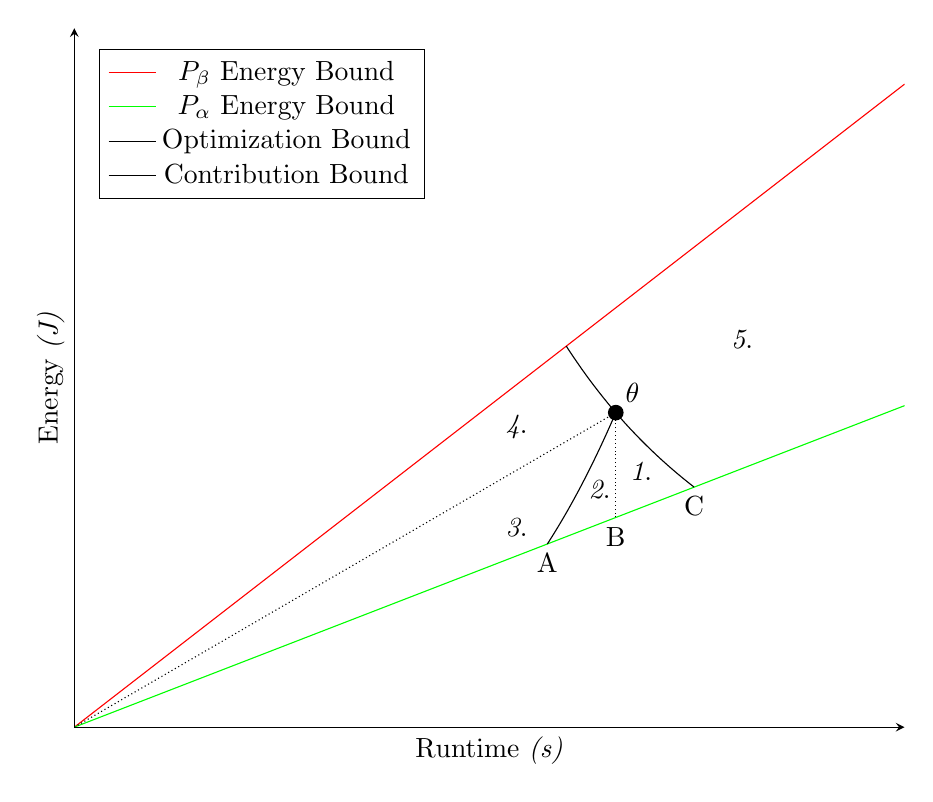
\begin{tikzpicture}

  \begin{axis}[ticks = none, 
    axis on top,
    axis x line=bottom,
    axis y line=left,
	xlabel={Runtime \emph{(s)}},
    ylabel={Energy \emph{(J)}},    
    xmin=0, xmax=46,
    ymin=0, ymax=3000,
    width=\linewidth,
    legend style={legend pos=north west}
    ]

    %% Model Parameters %%
    \pgfmathsetmacro{\baselinepower}{30} % NOP code
    \pgfmathsetmacro{\rooflinepower}{60}
    \pgfmathsetmacro{\codepower}{(\baselinepower + \rooflinepower) / 2}
    \pgfmathsetmacro{\codetime}{30}
    % Sadly, pgfplots sucks too much to calculate cube roots
    \pgfmathsetmacro{\anodex}{26.20741}
    \pgfmathsetmacro{\anodey}{\anodex * \baselinepower}
    \pgfmathsetmacro{\cnodex}{34.34143}
    \pgfmathsetmacro{\cnodey}{\cnodex * \baselinepower}
    \pgfmathsetmacro{\tnodex}{27.25681}
 
    %% Intermezzo Values %%
    \pgfmathsetmacro{\codeenergy}{\codepower * \codetime}
    \pgfmathsetmacro{\baselineenergy}{\baselinepower * \codetime}
    \pgfmathsetmacro{\rooflineenergy}{\rooflinepower * \codetime}
    \pgfmathsetmacro{\lowdisplayline}{(2 * \baselinepower + \codepower) / 3}
    \pgfmathsetmacro{\highdisplayline}{(1 * \rooflinepower + 1 * \codepower) / 2}

    % arguments: code power, code time, x - todo, apparently not supposed to do pgfmathparse
    \pgfmathdeclarefunction{metricbound}{3}{%
      \pgfmathparse{((#1 * #2^3) / #3^2)}%
    }
    \pgfmathdeclarefunction{definitionbound}{3}{%
      \pgfmathparse{((#1 / #2^3) * #3^4)}%
    }
     \pgfmathdeclarefunction{optimizationlimits}{3}{%
      \pgfmathparse{(min(metricbound(#1, #2, #3), definitionbound(#1, #2, #3)))}
    }

    % BETA ROOFLINE BOUND
    \addplot[color=red, name path=roofbound, domain=\pgfkeysvalueof{/pgfplots/xmin}:\pgfkeysvalueof{/pgfplots/xmax}] {\rooflinepower * x};
    \addlegendentry{$P_{\beta}$ Energy Bound}

    % ALPHA BASELINE BOUND 
    \addplot[color=green, name path=basebound, domain=\pgfkeysvalueof{/pgfplots/xmin}:\pgfkeysvalueof{/pgfplots/xmax}] {\baselinepower * x};
    \addlegendentry{$P_{\alpha}$ Energy Bound} 

    % Constant Time and Power Dashes
    \draw[densely dotted] ({axis cs:\codetime,\baselineenergy}) -- ({axis cs:\codetime,\codeenergy});
    \draw[densely dotted] ({axis cs:\pgfkeysvalueof{/pgfplots/xmin},\pgfkeysvalueof{/pgfplots/ymin}}) -- ({axis cs:\codetime,\codeenergy});
 

    \addplot[domain=\tnodex:\cnodex] { metricbound(\codepower, \codetime, x)};
    \addlegendentry{Optimization Bound}

    \addplot[domain=\anodex:\codetime] { definitionbound(\codepower, \codetime, x)};
    \addlegendentry{Contribution Bound}


    \node[circle,fill,inner sep=2pt] at (axis cs:\codetime,\codeenergy) {};
    \node[above right] at (axis cs:\codetime,\codeenergy) {$\theta$};
    \pgfmathsetmacro{\oneycoord}{\lowdisplayline * 31.4}
    \node at (axis cs:31.4,\oneycoord) {\textit1.};
    \pgfmathsetmacro{\twoycoord}{\lowdisplayline * 29.1}
    \node at (axis cs:29.1,\twoycoord) {\textit2.};
    \pgfmathsetmacro{\threeycoord}{\lowdisplayline * 24.5}
    \node at (axis cs:24.5,\threeycoord) {\textit3.};
    \pgfmathsetmacro{\fourycoord}{\highdisplayline * 24.5}
    \node at (axis cs:24.5,\fourycoord) {\textit4.};
    \pgfmathsetmacro{\fiveycoord}{\codepower * 37}
    \node at (axis cs:37,\fiveycoord) {\textit5.};
    
    \node [below] at ({axis cs:\anodex, \anodey}) {A};
    \node [below] at ({axis cs:\codetime,\baselineenergy}) {B};
    \node [below] at ({axis cs:\cnodex, \cnodey}) {C};
    %\node [below, name intersections={of=metric bound and baseline}] at (intersection-1) {C};


 \end{axis}
\end{tikzpicture}

\caption{POSE for $ED^2P$}
\label{fig:technique}
\end{figure}

The POSE heuristic is based on the concept of a \emph{Feasible Performance Envelope}.
We construct this by plotting lines of gradient $P_{max}$ and $P_{min}$ in \autoref{fig:technique}.
These values represent the maximum and minimum rate of power consumption which can occur during normal operation of the target platform. By definition the $\langle Runtime, Energy\rangle$ costs incurred by running any given code $\theta$ on the target platform must be represented somewhere within this envelope.

To constrain our search space further we now consider the metric we wish to reduce.
For two logically equivalent codes $\theta$ and $\lambda$, the transformation ${\theta \to \lambda}$ is a valid optimization with respect to a cost metric $M$ if and only if ${M(\lambda) < M(\theta)}$.
We plot a curve passing through $\theta$ linking all points with ${M(\lambda) = M(\theta)}$.
By definition any optimized versions of $\theta$ can only exist below this optimization bound.

Naturally the equation for the optimization bound depends on the metric we are optimizing for.
\autoref{fig:technique} shows the optimization bound for $ED^2P$.
The general form of this bound for the $E^mD^n$ family of metrics is derived as follows:
\begin{align}
E^mD^n(\lambda) &= E^mD^n(\theta) \nonumber \\
\implies {E_\lambda}^m &= \frac{{E_\theta}^m{D_\theta}^n}{{D_\lambda}^n} \nonumber \\
\implies E_\lambda &= (\frac{{E_\theta}^m{D_\theta}^n}{{D_\lambda}^n})^\frac{1}{m}
\label{eq:optimization}
\end{align}

Our second bound considers what it means to optimize code for reduced power draw. 
An optimization $\theta \to \lambda$ with respect to metric $M$ is a power optimization if the change in power draw it delivers is responsible for the majority of the reduction in $M$. We plot a curve through $\theta$ linking all points with the same ratio of contributions to $M$ from both power and runtime factors as our original code. All valid power optimizations must lie below this contribution bound. 

Again the equation for the contribution bound depends on the metric chosen. 
\autoref{fig:technique} shows the bound for $ED^2P$ whilst the general form for $E^mD^n$ metrics is:
\begin{align}
\frac{{P_{\lambda}}^m}{{D_{\lambda}}^{m+n}} &= \frac{{P_{\theta}}^m}{{D_{\theta}}^{m+n}} \nonumber \\
\implies {P_{\lambda}}^m &= \frac{{P_{\theta}}^m}{{D_{\theta}}^{m+n}} \times {D_\lambda}^{m+n} \nonumber \\ 
\implies {E_{\lambda}}^m &= \frac{{P_{\theta}}^m}{{D_{\theta}}^{m+n}} \times {D_\lambda}^{m+n+1} \nonumber \\ 
\implies E_{\lambda} &= (\frac{{P_{\theta}}^m}{{D_{\theta}}^{m+n}} \times {D_\lambda}^{m+n+1})^{\frac{1}{m}} 
\end{align}

Intuitively it makes sense to use the most appropriate tools while searching for optimizations.  If an optimization yields dramatic reductions in runtime with only minor reductions in power consumption then it is reasonable to classify it as a runtime optimization and state that conventional time-based profilers and performance engineering tools are better suited to finding it. It is the contribution bound which enables our model to make this distinction.

The bounds described thus far allow us to identify the area of the Energy/Runtime plane in which optimized versions of a given code exist and to subdivide this space into runtime and power optimizations. The final component of POSE is the Optimization Limit, which subdivides the runtime optimized area of the feasible performance envelope into those optimizations which may be outperformed by power optimizations, and those which strictly dominate all possible power optimizations.

The optimization limit is based on \autoref{eq:optimization} and closely mirrors the the optimization bound.
This limit connects all points with the same value for $M$ as a hypothetical maximally power optimized version of $\theta$. 
All points below this limit have lower values for $M$, and therefore any optimizations in this area strictly dominate any possible power optimizations. 

Along with lines of constant time and power draw, these bounds allow us to subdivide \autoref{fig:technique} into the following labelled areas:
\begin{enumerate}
\item Power-only optimizations
\item Power-mostly optimizations
\item Time-mostly optimizations
\item Time-only optimizations
\item Performance Degradation
\end{enumerate}

Two key strengths of POSE are its simplicity and generality.
Only three measurements are required to build this plot; the system's baseline power draw, $P_{min}$, and the time and energy to solution for the code to be optimized, $D_\theta$ and $E_\theta$ respectively.
The precise value of $P_{max}$ can be ommitted when optimizing for power draw as we need not consider any values greater than our initial $P_\theta$.
We also need to consider which metric we are optimizing. \autoref{fig:technique} is based on $ED^2P$, whilst \autoref{fig:multimetric-technique} demonstrates how the POSE optimization area varies with metric choice.

POSE offers a wealth of information to performance engineers.
The difference in energy between $\theta$ and intercept $B$ places an upper limit on the absolute amount of energy which can be saved by power optimization alone.
The value $M(A) - M(\theta)$ bounds the amount of improvement in our metric we can expect to see from power optimization.
The difference in runtime between intersect $C$ and $\theta$ represents the maximum increase in runtime we could feasibly trade off to achieve a slower yet more energy efficient code.
Finally, the value $D(\theta) / D(A)$ represents the smallest speed-up which delivers more benefit than power optimization is capable of.

\begin{figure}
\centering
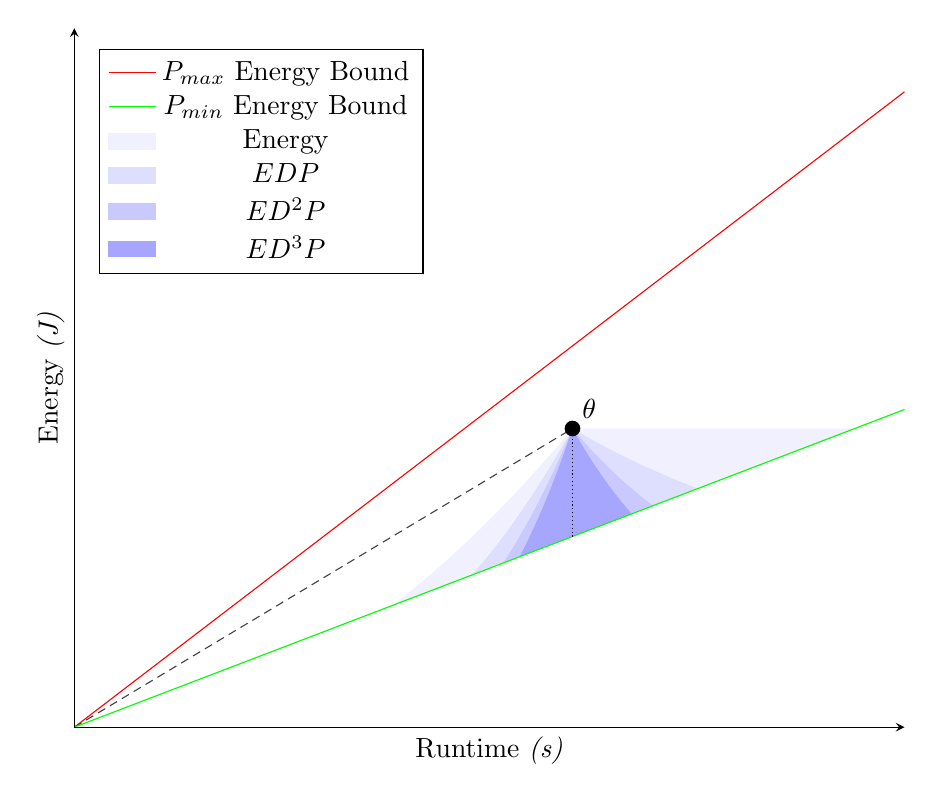
\begin{tikzpicture}
  \begin{axis}[ticks = none, 
    axis on top,
    axis x line=bottom,
    axis y line=left,
  	xlabel={Runtime \emph{(s)}},
    ylabel={Energy \emph{(J)}},    
    xmin=0, xmax=50,
    ymin=0, ymax=3300,
    width=\linewidth,
    legend style={legend pos=north west}
    ]

    %% Model Parameters %%
    \pgfmathsetmacro{\baselinepower}{30} % NOP code
    \pgfmathsetmacro{\rooflinepower}{60}
    \pgfmathsetmacro{\codepower}{47} 
    \pgfmathsetmacro{\codetime}{30}

    %% Intermezzo Values %%
    \pgfmathsetmacro{\codeenergy}{\codepower * \codetime}
    \pgfmathsetmacro{\baselineenergy}{\baselinepower * \codetime}
    \pgfmathsetmacro{\rooflineenergy}{\rooflinepower * \codetime}

    % arguments: code power, code time, x, n 
    \pgfmathdeclarefunction{metricbound}{4}{%
      \pgfmathparse{((#1 * #2^(#4 + 1)) / #3^#4)}%
    }
    \pgfmathdeclarefunction{definitionbound}{4}{%
      \pgfmathparse{((#1 / #2^(#4 + 1)) * #3^(#4 + 2))}%
    }
 
    % BETA ROOFLINE BOUND
    \addplot[color=red, domain=\pgfkeysvalueof{/pgfplots/xmin}:\pgfkeysvalueof{/pgfplots/xmax}] {\rooflinepower * x};
    \addlegendentry{$P_{max}$ Energy Bound}

    %const power diagonal
    \addplot[color=darkgray, densely dashed, name path=constpwr, forget plot, %forget plot prevents legend entry
            domain=\pgfkeysvalueof{/pgfplots/xmin}:\codetime] {\codepower * x}; 

    % ALPHA BASELINE BOUND 
    \addplot[color=green, name path=basebound, domain=\pgfkeysvalueof{/pgfplots/xmin}:\pgfkeysvalueof{/pgfplots/xmax}] {\baselinepower * x};
    \addlegendentry{$P_{min}$ Energy Bound} 

    % Constant Time vertical dots
    %vertical
    \draw[densely dotted] ({axis cs:\codetime,\baselineenergy}) -- ({axis cs:\codetime,\codeenergy});

    % Sadly, pgfplots sucks too much to calculate cube roots
    % Domain values are calculated with a ruby script in tools

    %% Energy Area %%
    \addplot[name path=energy, draw=none, domain=19.14894:47, forget plot]{ min(definitionbound(\codepower, \codetime, x, 0),metricbound(\codepower, \codetime, x, 0))};
    \addplot[blue!6] fill between[of=energy and basebound];
    \addlegendentry{Energy}

    %% Energy Delay Product Area %% 
    \addplot[name path=edp, draw=none, domain=23.96806:37.54997, forget plot] { min(definitionbound(\codepower, \codetime, x, 1),metricbound(\codepower, \codetime, x, 1))};
    \addplot[blue!13] fill between[of=edp and basebound];
    \addlegendentry{$EDP$}

    %% Energy Delay Squared Product Area ##
    \addplot[name path=edtwop, draw=none, domain=25.83028:34.84283, forget plot] { min(definitionbound(\codepower, \codetime, x, 2),metricbound(\codepower, \codetime, x, 2))};
    \addplot[blue!21] fill between[of=edtwop and basebound];
    \addlegendentry{$ED^2P$}

    %% Energy Delay Cubed Product Area ##
    \addplot[name path=edthreep, draw=none, domain=26.81496:33.56336, forget plot] { min(definitionbound(\codepower, \codetime, x, 3),metricbound(\codepower, \codetime, x, 3))};
    \addplot[blue!35] fill between[of=edthreep and basebound];
    \addlegendentry{$ED^3P$}




     \node[circle,fill,inner sep=2pt] at (axis cs:\codetime,\codeenergy) {};
    \node[above right] at (axis cs:\codetime,\codeenergy) {$\theta$};
  \end{axis}
\end{tikzpicture}

\caption{Multiple Metric Code Optimization Spaces}
\label{fig:multimetric-technique}
\end{figure}

  \section{Investigation}
\label{sec:investigation}
We now use POSE to investigate the CPU power consumption of codes from the Mantevo~\cite{heroux:2009aa} and Rodinia~\cite{che:2009aa} suites.
The applications we study are simplified versions of production codes intended for research purposes.
As such they exhibit relatively compact code bases and well understood behaviours while still providing represantative workloads.

CPU energy consumption accounts for a significant portion of the energy used by high performance systems~\cite{rong:2010aa} and is therefore a prime target for optimisation.
It can also be measured accurately on comodity hardware~\cite{hackenberg:2013aa} making it a suitable candidate for POSE modelling.

\subsection{CPU Power Consumption}
\label{ssec:cpupower}
Current processors are based on Complimentary Metal Oxide Semiconductor (CMOS) technology.
\autoref{eq:totpwr} separates the power draw of CMOS chips into its component parts, of which dynamic and leakage power are the most significant.
\begin{equation}
\label{eq:totpwr}
P_{tot} = P_{dyn} + P_{leak} + P_{other}
\end{equation}
Dynamic power is consumed when logic gates change state.
Leakage power exists because at microscopic scales the insulating properties of silicon break down, allowing some current to escape even when gates remain inactive.
Other forms of power dissipation exist, however their effects are relatively minor \cite{kaxiras:2008aa}.
\begin{gather}
P_{dyn} \propto CV^{2}Af \label{eq:dynpwr} \\
P_{leak} = V \times I_{leak} \label{eq:staticpwr}
\end{gather}
\autoref{eq:dynpwr} is a common approximation for dynamic power in which $C$ denotes load capacitance, $V$ the supply voltage, $A$ the activity factor and $f$ the clock frequency.
\autoref{eq:staticpwr} is a simplified expression for leakage power which exploits the fact that leakage current $I_{leak}$ is invariant to processor workload~\cite{kim:2003aa}.

Activity factor captures the fraction of logic elements which change state each clock cycle.
Frequency and supply voltage vary in tandem, taking values from a set of $(frequency, voltage)$ pairs known as P-states.
Dynamic Voltage and Frequency Scaling (DVFS) selects a P-state based on workload, or places the CPU into an energy saving mode if no work is available.
Finally, capacitance and leakage current are constants dictated by hardware design.

Processor architecture also plays a significant roll in determining total power consumption.
Each core in a multicore architecture operates independantly with its own activity factor and in some cases P-state.
As a result, \autoref{eq:totpwr} should be summed across all cores to arrive at a value for the entire processor.

\subsection{Feasible Performance Envelope}
The first step in applying POSE is to construct a feasible performance envelope.
Manufacturers publish the power dissipation figures of their hardware, however these values are usually conservative for safety reasons.
POSE works best when the maximum and minimum power bounds are as tight as possible.
We therefore determine $P_{\max}$ and $P_{\min}$ empirically.

We describe power benchmarks using $(S,A,C)$ tuples with P-state $S$, activity factor $A$ and active core count $C$; the three properties which link software to CPU power draw.
Our $P_{min}$ and $P_{max}$ benchmarks should reflect the range of values these properties can take for a given code $\theta$.
We formalise this notion in \autoref{eq:pbench}.
\begin{align}
  \label{eq:pbench}
  \begin{split}
    P_{min} &= (S_{min}, A_{min}, C_{min}~\vert~\theta), \\
    P_{max} &= (S_{max}, A_{max}, C_{max}~\vert~\theta) 
  \end{split}
\end{align}
The values of $S$, $A$, and $C$ depend on the code and the nature of the optimisations being considered.
POSE models for inherently serial codes should be constructed using single threaded benchmarks where $C_{min} = C_{max} = 1$, for example.

The \texttt{cpufrequtils} package allows us to override DVFS and manually set the desired P-state $S$.
We control the number of active cores $C$ by specifying the number of threads used by our benchmarking routines and pinning each one to its own core to prevent migration.
The only remaining property is activity factor, which is influenced by benchmark code.

\begin{figure}[ht]
\centering
\lstset{basicstyle=\ttfamily\footnotesize\bfseries, frame=tb} %small bold text, lines top and bottom
\lstinputlisting[]{lst/alpha_benchmark.c}
\caption{Activity Factor $\alpha$ Benchmark Code}
\label{fig:microbench}
\end{figure}

We define the range of values that $A$ can take for some fixed $S$ and $C$ as $[\alpha,~\beta]$ where $0 < \alpha < \beta < 1$.
Our code for targeting activity factor $\alpha$ is given in \autoref{fig:microbench}.
This benchmark executes a single \texttt{jmp} instruction each clock cycle, preventing instruction pipelining.
It performs no floating point or integer calculations and no memory accesses whilst keeping control logic to a minimum.

Any non-trivial code will perform more work than our benchmark and will therefore have a higher activity factor.
The only exception occurs when applications are blocked for long periods, allowing the processor to enter an idle state.
This can be addressed by adding delays to the benchmark if necessary.

FIRESTARTER~\cite{hackenberg:2013ab} serves as our benchmark for activity factor $\beta$.
This tool is designed to trigger near-peak power consumption across a range of x86\_64 processors.
It consists of hand optimised assembly routines which raise activity factor above the level achievable with high level languages.
Prime95 and Linpack were also evaluated as potential $\beta$ benchmarks however they were consistently outperformed by FIRESTARTER.

The benchmark parameter space is small enough to fully characterise a processor by measuirng all $(S,A,C)$ configurations.
Benchmarking runs lasted for 120 seconds to allow enough time for power readings to stabilize.
We extended the Unix \texttt{time} binary to gather power consumption figures using Intel's Running Average Power Limit (RAPL) technology~\cite{david:2010aa}.
The techniques described in \cite{hahnel:2012aa} were used to promote measurement accuracy.
Results are presented in \autoref{tab:fpe_params}, which identifies P-states by their frequency component.

\begin{table}
\centering
\caption{Feasible Performance Envelope Parameters (W)}
\label{tab:fpe_params}
\input{tab/tex/fpe_params.tex}
\end{table}

\subsection{POSE Models for Code Optimisation}
Having characterised our system we now proceed to build POSE models for applications in the Mantevo and Rodinia suites.
These codes were compiled with ICC version 14.0.0.
Codes were run with default configurations where available.
The energy and runtime costs associated with each code is given in \autoref{tab:code_metrics}.

\begin{table}
\centering
\caption{Code Energy Measurements}
\label{tab:code_metrics}
\input{tab/tex/code_metrics.tex}
\end{table}

All codes evaluated ran in parallel across four cores.
They also spent a negligible amount of time waiting for resources. 
This allowed the CPU to run at its maximum supported frequency of 3.2 GHz.
For the first stage of this investigation we disregard any optimisations which reduce parallelism ($C < 4$) or reduce processor throughput ($S < 3.2GHz$).
The benchmark configurations used were $(\text{3.2 GHz}, \alpha, 4)$ for $P_{min}$ and $(\text{3.2 GHz}, \beta, 4)$ for $P_{max}$, yielding power draws of 26.88W and 49.61W respectively.

\begin{table}
  \setlength{\tabcolsep}{.5em}
  \caption{$E^1t^2$ POSE Points}
  \begin{subtable}{\textwidth}
  \centering
  \caption{Time (s)}
  \input{tab/tex/code_pose_time.tex}
  \end{subtable}
  \begin{subtable}{\textwidth}
  \centering
  \caption{Energy (J)}
  \input{tab/tex/code_pose_energy.tex}
  \end{subtable}
  \label{tab:pose_params}
\end{table}

\autoref{tab:pose_params} summarises the POSE models constructed for each code.
The remainder of this section focusses on MiniMD and LavaMD as the two codes which represent the extremes of power consumption.
POSE models for these two codes are reproduced graphically in \autoref{fig:minimd_pose} and \autoref{fig:lavamd_pose}.
When comparing these diagrams it is readily apparent that LavaMD offers far more scope for power optimisation than MiniMD, which offers virtually none. 
POSE provides the following insights for LavaMD:
\begin{itemize}
  \item At most 353.36J can be saved by reducing power consumption
  \item The maximum slowdown from energy optimisation is 4.12s
  \item The lowest $E^1t^2$ value from power optimisation is 6332609
  \begin{itemize}
  \item Corresponding to a 30.59\% improvement
  \end{itemize}
  \item A speedup of 8.77s, or 1.15x, strictly outperforms $\theta$
  \item A speedup of 15.29s, or 1.30x, strictly outperforms any power optimisation
\end{itemize}

\begin{figure}[t]%
  \providecommand{\plotwidth}{.95\linewidth}
  \begin{subfigure}[t]{.5\linewidth}%
    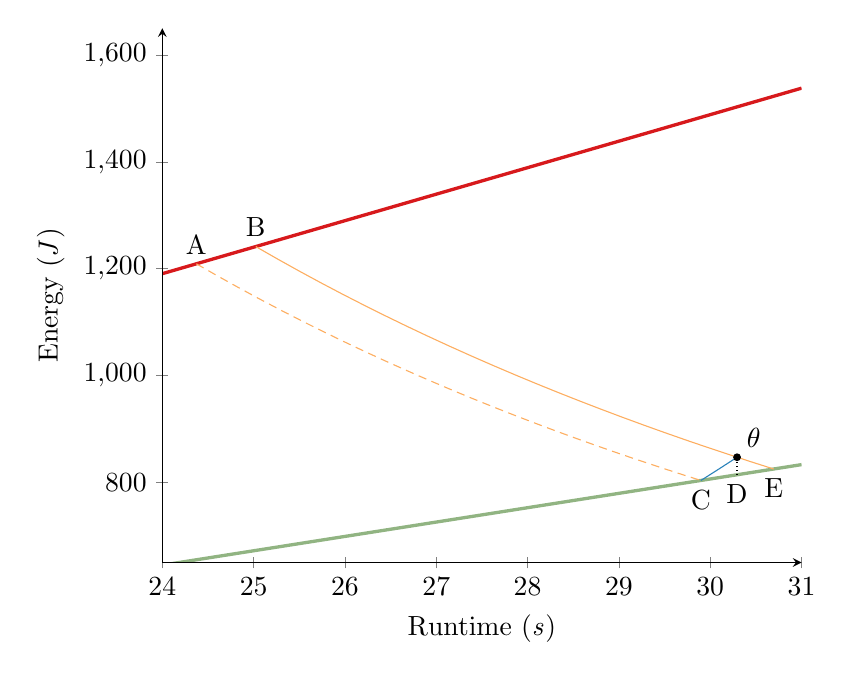
\begin{tikzpicture}
  \begin{axis}[
    axis on top,
    axis x line=bottom,
    axis y line=left,
    xlabel={Runtime (\emph{s})},
    ylabel={Energy (\emph{J})},    
    xmin=24, xmax=31,
    ymin=650, ymax=1650,
    width=0.80\linewidth,
    legend columns=3,
    legend to name=minimd:legend,
    legend style={/tikz/every even column/.append style={column sep=0.2cm}} % space out columns a bit
    ]

    %% Model Parameters %%
    \pgfmathsetmacro{\baselinepower}{26.876067}
    \pgfmathsetmacro{\rooflinepower}{49.60612}
    \pgfmathsetmacro{\codepower}{27.95947000000066} 
    \pgfmathsetmacro{\codetime}{30.293834}
    \pgfmathsetmacro{\codeenergy}{846.999542908}
    \pgfmathsetmacro{\energyexp}{1.0}
    \pgfmathsetmacro{\timeexp}{2.0}

    % Sadly, pgfplots sucks too much to calculate cube roots
    % These values are calculated with a ruby script in tools
    \pgfmathsetmacro{\blnodex}{29.897382525363728}
    \pgfmathsetmacro{\brnodex}{30.69554258273286}
    \pgfmathsetmacro{\trnodex}{25.0237350439618}
    \pgfmathsetmacro{\tlnodex}{24.373056016397907}

    %% Intermezzo Values %%
    \pgfmathsetmacro{\brnodey}{\brnodex * \baselinepower}
    \pgfmathsetmacro{\blnodey}{\blnodex * \baselinepower}
    \pgfmathsetmacro{\tlnodey}{\tlnodex * \rooflinepower}
    \pgfmathsetmacro{\trnodey}{\trnodex * \rooflinepower}
    \pgfmathsetmacro{\codeenergy}{\codepower * \codetime}
    \pgfmathsetmacro{\baselineenergy}{\baselinepower * \codetime}

    % arguments: code power, code time, x - todo, apparently not supposed to do pgfmathparse
    \pgfmathdeclarefunction{metricbound}{3}{%
      \pgfmathparse{((#1 * #2^3) / #3^2)}%
    }
    \pgfmathdeclarefunction{definitionbound}{3}{%
      \pgfmathparse{((#1 / #2^3) * #3^4)}%
    }

   % BETA ROOFLINE BOUND 
    \addplot[color=printred, very thick, domain=\pgfkeysvalueof{/pgfplots/xmin}:\pgfkeysvalueof{/pgfplots/xmax}] {\rooflinepower * x};
    \addlegendentry{$P_{max}$ Energy Bound}

    % ALPHA BASELINE BOUND 
    \addplot[color=printgreen, very thick, domain=\pgfkeysvalueof{/pgfplots/xmin}:\pgfkeysvalueof{/pgfplots/xmax}] {\baselinepower * x};
    \addlegendentry{$P_{min}$ Energy Bound} 

    \addplot[color=printorange, domain=\trnodex:\brnodex] { metricbound(\codepower, \codetime, x)};
    \addlegendentry{Optimisation Bound}

    \addplot[color=printblue, domain=\blnodex:\codetime] { definitionbound(\codepower, \codetime, x)};
    \addlegendentry{Contribution Bound}

    \addplot[color=printorange, densely dashed, domain=\tlnodex:\blnodex] {metricbound(\baselinepower, \blnodex, x)};
    \addlegendentry{Optimisation Limit}

    % Constant Time (Vertical) dotted line
    \draw[densely dotted] ({axis cs:\codetime,\baselineenergy}) -- ({axis cs:\codetime,\codeenergy});

    \node[circle,fill,inner sep=1pt] at (axis cs:\codetime,\codeenergy) {};
    \node[above right] at (axis cs:\codetime,\codeenergy) {$\theta$};
    
    \node [above] at ({axis cs:\tlnodex, \tlnodey}) {A};
    \node [above] at ({axis cs:\trnodex, \trnodey}) {B};
    \node [below] at ({axis cs:\blnodex, \blnodey}) {C};
    \node [below] at ({axis cs:\codetime,\baselineenergy}) {D};
    \node [below] at ({axis cs:\brnodex, \brnodey}) {E};
 \end{axis}
\end{tikzpicture}
%
    \caption{MiniMD}%
    \label{fig:minimd_pose}
  \end{subfigure}%
  \begin{subfigure}[t]{.5\linewidth}%
    \begin{tikzpicture}
  \providecommand{\plotwidth}{\linewidth}
  \begin{axis}[
    axis on top,
    axis x line=bottom,
    axis y line=left,
  	xlabel={Runtime \emph{(s)}},
    ylabel={Energy \emph{(J)}},    
    xmin=50, xmax=75,
    ymin=1200, ymax=4000,
    width=\plotwidth,
    legend to name=lavamd:legend
    ]

    %% Model Parameters %%
    \pgfmathsetmacro{\baselinepower}{26.876067}
    \pgfmathsetmacro{\rooflinepower}{43.570651}
    \pgfmathsetmacro{\codepower}{32.259372}
    \pgfmathsetmacro{\codetime}{65.640072}
    % Sadly, pgfplots sucks too much to calculate cube roots
    % These values are calculated with a ruby script in tools
    \pgfmathsetmacro{\brnodex}{69.75881800188515}
    \pgfmathsetmacro{\blnodex}{61.764507707810466}
    \pgfmathsetmacro{\trnodex}{59.38220710689976}
    \pgfmathsetmacro{\tlnodex}{52.57704894686994}
    
    %% Intermezzo Values %%
    \pgfmathsetmacro{\brnodey}{\brnodex * \baselinepower}
    \pgfmathsetmacro{\blnodey}{\blnodex * \baselinepower}
    \pgfmathsetmacro{\tlnodey}{\tlnodex * \rooflinepower}
    \pgfmathsetmacro{\trnodey}{\trnodex * \rooflinepower}
    \pgfmathsetmacro{\codeenergy}{\codepower * \codetime}
    \pgfmathsetmacro{\baselineenergy}{\baselinepower * \codetime}

    % arguments: code power, code time, x - todo, apparently not supposed to do pgfmathparse
    \pgfmathdeclarefunction{metricbound}{3}{%
      \pgfmathparse{((#1 * #2^3) / #3^2)}%
    }
    \pgfmathdeclarefunction{definitionbound}{3}{%
      \pgfmathparse{((#1 / #2^3) * #3^4)}%
    }

    % BETA ROOFLINE BOUND 
    \addplot[color=red, domain=\pgfkeysvalueof{/pgfplots/xmin}:\pgfkeysvalueof{/pgfplots/xmax}] {\rooflinepower * x};
    \addlegendentry{$P_{max}$ Energy Bound}

    % ALPHA BASELINE BOUND 
    \addplot[color=green, domain=\pgfkeysvalueof{/pgfplots/xmin}:\pgfkeysvalueof{/pgfplots/xmax}] {\baselinepower * x};
    \addlegendentry{$P_{min}$ Energy Bound} 

    \addplot[color=orange, domain=\trnodex:\brnodex] { metricbound(\codepower, \codetime, x)};
    \addlegendentry{Optimisation Bound}

    \addplot[color=blue!80, domain=\blnodex:\codetime] { definitionbound(\codepower, \codetime, x)};
    \addlegendentry{Contribution Bound}

    \addplot[color=orange, dashed, domain=\tlnodex:\blnodex] {metricbound(\baselinepower, \blnodex, x)};
    \addlegendentry{Optimisation Limit}

    % Constant Time (Vertical) dotted line
    \draw[densely dotted] ({axis cs:\codetime,\baselineenergy}) -- ({axis cs:\codetime,\codeenergy});

    \node[circle,fill,inner sep=2pt] at (axis cs:\codetime,\codeenergy) {};
    \node[above right] at (axis cs:\codetime,\codeenergy) {$\theta$};
    
    \node [above] at ({axis cs:\tlnodex, \tlnodey}) {A};
    \node [above] at ({axis cs:\trnodex, \trnodey}) {B};
    \node [below] at ({axis cs:\blnodex, \blnodey}) {C};
    \node [below] at ({axis cs:\codetime,\baselineenergy}) {D};
    \node [below] at ({axis cs:\brnodex, \brnodey}) {E};
 \end{axis}
\end{tikzpicture}
%
    \caption{LavaMD}%
    \label{fig:lavamd_pose}
  \end{subfigure}%
  \begin{center}%
    \ref{minimd:legend}%
  \end{center}%
  \caption{$E^1t^2$ POSE comparrison}%
  \label{fig:comparrison}%
\end{figure}

\begin{figure}[t]%
\begin{subfigure}[t]{.5\linewidth}%
\centering%
\@ifundefined{pstateminimdtable}{%
  \pgfplotstableread[col sep=comma]{plot/minimd-pstates/data/pstate_power_4_cores.csv}\pstateminimdtable
}{}

\begin{tikzpicture}
  \begin{axis}[
    width=0.75\linewidth,
    axis on top,
    axis x line=bottom,
    axis y line=left,
    xlabel={Runtime (\emph{s})},
    ylabel={Energy (\emph{J})},    
    xmin=20, xmax=65,
    ymin=200, ymax=1200,
    legend columns=2,
    legend to name=minimd-pstate:legend,
    legend style={/tikz/every even column/.append style={column sep=0.2cm}} % space out columns a bit
    ]

    % arguments: code power, code time, x, n 
    \pgfmathdeclarefunction{metricbound}{4}{%
      \pgfmathparse{((#1 * #2^(#4 + 1)) / #3^#4)}%
    }
    \pgfmathdeclarefunction{definitionbound}{4}{%
      \pgfmathparse{((#1 / #2^(#4 + 1)) * #3^(#4 + 2))}%
    }

    %%
    \pgfmathsetmacro{\codetime}{31.160996}
    \pgfmathsetmacro{\codepower}{26.555410070974624}
    \pgfmathsetmacro{\blnodex}{24.876044579784466}
    \addplot[black, densely dotted, domain=\blnodex:\codetime, forget plot] {definitionbound(\codepower, \codetime, x, 2)};

    %%
    \pgfmathsetmacro{\codetime}{32.221644}
    \pgfmathsetmacro{\codepower}{25.19066851461707}
    \pgfmathsetmacro{\blnodex}{26.17914532437151}
    \addplot[black, densely dotted, domain=\blnodex:\codetime, forget plot] {definitionbound(\codepower, \codetime, x, 2)};

    %%
    \pgfmathsetmacro{\codetime}{33.189564}
    \pgfmathsetmacro{\codepower}{24.052689996168674}
    \pgfmathsetmacro{\blnodex}{27.384280155637242}
    \addplot[black, densely dotted, domain=\blnodex:\codetime, forget plot] {definitionbound(\codepower, \codetime, x, 2)};

    %%
    \pgfmathsetmacro{\codetime}{35.548669}
    \pgfmathsetmacro{\codepower}{21.708309894809283}
    \pgfmathsetmacro{\blnodex}{30.35072062021389}
    \addplot[black, densely dotted, domain=\blnodex:\codetime, forget plot] {definitionbound(\codepower, \codetime, x, 2)};

    %%
    \pgfmathsetmacro{\codetime}{36.852917}
    \pgfmathsetmacro{\codepower}{20.791885293639034}
    \pgfmathsetmacro{\blnodex}{31.919904165043228}
    \addplot[black, densely dotted, domain=\blnodex:\codetime, forget plot] {definitionbound(\codepower, \codetime, x, 2)};

    %%
    \pgfmathsetmacro{\codetime}{38.225746}
    \pgfmathsetmacro{\codepower}{19.926273930664426}
    \pgfmathsetmacro{\blnodex}{33.58161699951163}
    \addplot[black, densely dotted, domain=\blnodex:\codetime, forget plot] {definitionbound(\codepower, \codetime, x, 2)};

    %%
    \pgfmathsetmacro{\codetime}{39.720356}
    \pgfmathsetmacro{\codepower}{19.032817706870503}
    \pgfmathsetmacro{\blnodex}{35.432334683311204}
    \addplot[black, densely dotted, domain=\blnodex:\codetime, forget plot] {definitionbound(\codepower, \codetime, x, 2)};

    %%
    \pgfmathsetmacro{\codetime}{41.430395}
    \pgfmathsetmacro{\codepower}{18.26008617586195}
    \pgfmathsetmacro{\blnodex}{37.47190734697387}
    \addplot[black, densely dotted, domain=\blnodex:\codetime, forget plot] {definitionbound(\codepower, \codetime, x, 2)};

    %%
    \pgfmathsetmacro{\codetime}{45.85507}
    \pgfmathsetmacro{\codepower}{16.61222678321067}
    \pgfmathsetmacro{\blnodex}{42.802165661611}
    \addplot[black, densely dotted, domain=\blnodex:\codetime, forget plot] {definitionbound(\codepower, \codetime, x, 2)};

    %%
    \pgfmathsetmacro{\codetime}{49.7305}
    \pgfmathsetmacro{\codepower}{15.67846259337831}
    \pgfmathsetmacro{\blnodex}{47.323406701270244}
    \addplot[black, densely dotted, domain=\blnodex:\codetime, forget plot] {definitionbound(\codepower, \codetime, x, 2)};

    %%
    \pgfmathsetmacro{\codetime}{52.358683}
    \pgfmathsetmacro{\codepower}{15.137478343372388}
    \pgfmathsetmacro{\blnodex}{50.41098720057872}
    \addplot[black, densely dotted, domain=\blnodex:\codetime, forget plot] {definitionbound(\codepower, \codetime, x, 2)};

    %%
    \pgfmathsetmacro{\codetime}{55.340763}
    \pgfmathsetmacro{\codepower}{14.650088958838532}
    \pgfmathsetmacro{\blnodex}{53.866578212248804}
    \addplot[black, densely dotted, domain=\blnodex:\codetime, forget plot] {definitionbound(\codepower, \codetime, x, 2)};

    %%
    \pgfmathsetmacro{\codetime}{58.637567}
    \pgfmathsetmacro{\codepower}{14.09304050763225}
    \pgfmathsetmacro{\blnodex}{57.81786383949271}
    \addplot[black, densely dotted, domain=\blnodex:\codetime, forget plot] {definitionbound(\codepower, \codetime, x, 2)};


    %% Model Parameters %%
    \pgfplotstablegetelem{0}{Runtime}\of{\pstateminimdtable}
    \pgfmathsetmacro{\codetime}{\pgfplotsretval} 
    \pgfplotstablegetelem{0}{Energy}\of{\pstateminimdtable}
    \pgfmathsetmacro{\codeenergy}{\pgfplotsretval} 
    \pgfmathsetmacro{\baselinepower}{13.510238}

    %% Intermezzo Values %%
    \pgfmathsetmacro{\codepower}{\codeenergy / \codetime}



    % ALPHA BASELINE BOUND 
    \addplot[color=printgreen, very thick, name path=basebound, domain=\pgfkeysvalueof{/pgfplots/xmin}:\pgfkeysvalueof{/pgfplots/xmax}] {\baselinepower * x};
    \addlegendentry{$P_{min}$ Energy Bound} 


    %% 3.2 GHz start point
    \pgfmathsetmacro{\blnodex}{23.77199310523716}
    \pgfmathsetmacro{\brnodex}{38.6049404590049}
    \addplot[name path=edpdef, darkgray, thick, domain=\blnodex:\codetime, forget plot] {definitionbound(\codepower, \codetime, x, 2)};
    \addplot[name path=edpopt, darkgray, thick, domain=\codetime:\brnodex] {metricbound(\codepower, \codetime, x, 2)};
    \addlegendentry{3.2 GHz POSE}

    % 2.2 GHz non-overlapping pose
    \pgfmathsetmacro{\codetime}{43.161913}
    \pgfmathsetmacro{\codepower}{17.552650110758528}
    \pgfmathsetmacro{\blnodex}{39.55555231782452}
    \pgfmathsetmacro{\brnodex}{47.097072968441026}
    \addplot[name path=edpdef, gray, thick, domain=\blnodex:\codetime, forget plot] {definitionbound(\codepower, \codetime, x, 2)};
    \addplot[name path=edpopt, gray, thick, domain=\codetime:\brnodex] {metricbound(\codepower, \codetime, x, 2)};
    \addlegendentry{First Non-Overlapping POSE}
    
    %% PState progression
    \tikzset{ every pin edge/.append style={thick} }
    \addplot[mark=x, black, only marks] table[x=Runtime,y=Energy, trim cells=true] {\pstateminimdtable}
      node[pos=0.0, pin=above:3.2 GHz]{}
      node[pos=1.0, pin=above:1.6 GHz]{}
      node[pos=0.64285714285, pin=above:2.2 GHz]{} % pos is elem index / rows - 1 (zero indexed)
      % How to specify pin length (.15cm) and angle (120)
      %node[pos=0.5745, pin={[pin distance=0.15cm] 120:2.2 GHz}]{}
    ;
    \addlegendentry{P-state Measurement}
 \end{axis}
\end{tikzpicture}
%
\caption{MiniMD}%
\end{subfigure}%
\begin{subfigure}[t]{.5\linewidth}%
\@ifundefined{pstatelavamdtable}{%
  \pgfplotstableread[col sep=comma]{plot/lavamd-pstates/data/pstate_power_4_cores.csv}\pstatelavamdtable
}{}

\begin{tikzpicture}
  \begin{axis}[
    width=0.95\linewidth,
    axis on top,
    axis x line=bottom,
    axis y line=left,
  	xlabel={Runtime \emph{(s)}},
    ylabel={Energy \emph{(J)}},    
    xmin=0, xmax=140,
    ymin=0, ymax=3800,
    legend columns=2,
    legend to name=lavamd-pstate:legend,
    legend style={/tikz/every even column/.append style={column sep=0.2cm}} % space out columns a bit
    ]

    %% Model Parameters %%
    \pgfplotstablegetelem{0}{Runtime}\of{\pstatelavamdtable}
    \pgfmathsetmacro{\codetime}{\pgfplotsretval} 
    \pgfplotstablegetelem{0}{Energy}\of{\pstatelavamdtable}
    \pgfmathsetmacro{\codeenergy}{\pgfplotsretval} 
    \pgfmathsetmacro{\baselinepower}{13.510238}

    %% Intermezzo Values %%
    \pgfmathsetmacro{\codepower}{\codeenergy / \codetime}

    % arguments: code power, code time, x, n 
    \pgfmathdeclarefunction{metricbound}{4}{%
      \pgfmathparse{((#1 * #2^(#4 + 1)) / #3^#4)}%
    }
    \pgfmathdeclarefunction{definitionbound}{4}{%
      \pgfmathparse{((#1 / #2^(#4 + 1)) * #3^(#4 + 2))}%
    }

    % ALPHA BASELINE BOUND 
    \addplot[color=green, name path=basebound, domain=\pgfkeysvalueof{/pgfplots/xmin}:\pgfkeysvalueof{/pgfplots/xmax}] {\baselinepower * x};
    \addlegendentry{$P_{min}$ Energy Bound} 


    %% 3.2 GHz start point
    \pgfmathsetmacro{\brnodex}{87.73374843784023}
    \pgfmathsetmacro{\blnodex}{49.11016716922632}
    \addplot[name path=edpdef, draw=none, domain=\blnodex:\codetime+1, forget plot] {definitionbound(\codepower, \codetime, x, 2)};
    \addplot[name path=edpopt, draw=none, domain=\codetime-1:\brnodex, forget plot] {metricbound(\codepower, \codetime, x, 2)};

    \path[name path=edpspace,
      intersection segments={
        of=edpdef and edpopt,
        sequence=A0 -- B1,
      }
      ]; 
    \addplot[blue!20] fill between[of=edpspace and basebound]; 
    \addlegendentry{3.2 GHz POSE}

    %% PState progression
    \addplot[mark=x, black] table[x=Runtime,y=Energy, trim cells=true] {\pstatelavamdtable}
      node[pos=0.0, pin=left:3.2 GHz]{}
      node[pos=1.0, pin=95:1.6 GHz]{}
      node[pos=0.636, pin={[pin distance=0.15cm] above:2.1 GHz}]{}
    ;
    \addlegendentry{P-State Progression}


    %%
    \pgfmathsetmacro{\codetime}{67.788671}
    \pgfmathsetmacro{\codepower}{30.534496154969613}
    \pgfmathsetmacro{\blnodex}{51.65525781584337}
    \addplot[name path=edpdef, gray, densely dashed, domain=\blnodex:\codetime, forget plot] {definitionbound(\codepower, \codetime, x, 2)};

    %%
    \pgfmathsetmacro{\codetime}{69.909725}
    \pgfmathsetmacro{\codepower}{28.972621505806238}
    \pgfmathsetmacro{\blnodex}{54.21207070239038}
    \addplot[name path=edpdef, gray, densely dashed, domain=\blnodex:\codetime, forget plot] {definitionbound(\codepower, \codetime, x, 2)};

    %%
    \pgfmathsetmacro{\codetime}{72.820343}
    \pgfmathsetmacro{\codepower}{27.23156518227331}
    \pgfmathsetmacro{\blnodex}{57.647815146592066}
    \addplot[name path=edpdef, gray, densely dashed, domain=\blnodex:\codetime, forget plot] {definitionbound(\codepower, \codetime, x, 2)};

    %%
    \pgfmathsetmacro{\codetime}{78.83738}
    \pgfmathsetmacro{\codepower}{24.363863791516156}
    \pgfmathsetmacro{\blnodex}{64.76958711476986}
    \addplot[name path=edpdef, gray, densely dashed, domain=\blnodex:\codetime, forget plot] {definitionbound(\codepower, \codetime, x, 2)};

    %%
    \pgfmathsetmacro{\codetime}{80.443575}
    \pgfmathsetmacro{\codepower}{23.569310575766927}
    \pgfmathsetmacro{\blnodex}{66.82363092159444}
    \addplot[name path=edpdef, gray, densely dashed, domain=\blnodex:\codetime, forget plot] {definitionbound(\codepower, \codetime, x, 2)};

    %%
    \pgfmathsetmacro{\codetime}{83.583275}
    \pgfmathsetmacro{\codepower}{22.42571518045925}
    \pgfmathsetmacro{\blnodex}{70.59245458487962}
    \addplot[name path=edpdef, gray, densely dashed, domain=\blnodex:\codetime, forget plot] {definitionbound(\codepower, \codetime, x, 2)};

    %%
    \pgfmathsetmacro{\codetime}{87.25231}
    \pgfmathsetmacro{\codepower}{21.415643975500476}
    \pgfmathsetmacro{\blnodex}{74.83203474018039}
    \addplot[name path=edpdef, gray, densely dashed, domain=\blnodex:\codetime, forget plot] {definitionbound(\codepower, \codetime, x, 2)};

    %%
    \pgfmathsetmacro{\codetime}{90.581583}
    \pgfmathsetmacro{\codepower}{20.54295973167084}
    \pgfmathsetmacro{\blnodex}{78.77224707386881}
    \addplot[name path=edpdef, gray, densely dashed, domain=\blnodex:\codetime, forget plot] {definitionbound(\codepower, \codetime, x, 2)};

    %%
    \pgfmathsetmacro{\codetime}{95.357508}
    \pgfmathsetmacro{\codepower}{19.637888418812288}
    \pgfmathsetmacro{\blnodex}{84.1803958382032}
    \addplot[name path=edpdef, gray, densely dashed, domain=\blnodex:\codetime, forget plot] {definitionbound(\codepower, \codetime, x, 2)};

    %%
    \pgfmathsetmacro{\codetime}{99.502899}
    \pgfmathsetmacro{\codepower}{18.820670933416725}
    \pgfmathsetmacro{\blnodex}{89.0932975465577}
    \addplot[name path=edpdef, red, densely dashed, domain=\blnodex:\codetime] {definitionbound(\codepower, \codetime, x, 2)};
    \addlegendentry{Optimisation Cutoff}
    %%
    \pgfmathsetmacro{\codetime}{109.970804}
    \pgfmathsetmacro{\codepower}{17.334285425429826}
    \pgfmathsetmacro{\blnodex}{101.20370662532102}
    \addplot[name path=edpdef, gray, densely dashed, domain=\blnodex:\codetime, forget plot] {definitionbound(\codepower, \codetime, x, 2)};

    %%
    \pgfmathsetmacro{\codetime}{115.469869}
    \pgfmathsetmacro{\codepower}{16.703561489274747}
    \pgfmathsetmacro{\blnodex}{107.58539357794623}
    \addplot[name path=edpdef, gray, densely dashed, domain=\blnodex:\codetime, forget plot] {definitionbound(\codepower, \codetime, x, 2)};

    %%
    \pgfmathsetmacro{\codetime}{123.182269}
    \pgfmathsetmacro{\codepower}{16.060352379123653}
    \pgfmathsetmacro{\blnodex}{116.28334319474206}
    \addplot[name path=edpdef, gray, densely dashed, domain=\blnodex:\codetime, forget plot] {definitionbound(\codepower, \codetime, x, 2)};

    %%
    \pgfmathsetmacro{\codetime}{130.924339}
    \pgfmathsetmacro{\codepower}{15.486518591474423}
    \pgfmathsetmacro{\blnodex}{125.09985043035239}
    \addplot[name path=edpdef, gray, densely dashed, domain=\blnodex:\codetime, forget plot] {definitionbound(\codepower, \codetime, x, 2)};
  \end{axis}
\end{tikzpicture}
%
\caption{LavaMD}%
\end{subfigure}%
\begin{center}%
\ref{minimd-pstate:legend}%
\end{center}%
\caption{$E^1t^2$ POSE for P-state Optimisation}%
\label{fig:pstates}%
\end{figure}%


\subsection{POSE Models for Frequency Scaling}
DVFS impacts performance in a non-linear fashion. \todo{cite critical power slope}
Codes prone to external bottlenecks like memory bandwidth or I/O latency typically leave the CPU underutilized.
In these cases reducing the clock frequency can deliver energy savings without significant performance degradation. \todo{cite 




Research has shown that in these cases energy can be saved with 

be made 

http://citeseerx.ist.psu.edu/viewdoc/download?doi=10.1.1.60.8266&rep=rep1&type=pdf

In these cases



DVFS attempts to select the most appropriate P-state for the current workflow.
That said, its reactive and coarse grained nature mean that its decisions can be sub-optimal decisions.
Optimal frequency schedule, so that the processor only works as fast as 

In this case CPU frequency can be reduced without adversely affecting performance.
Conversely, if the CPU itself is a performance bottleneck, the maximum frequency possible should be selected.



e the balance of pressures on external bottlenecks.


If instruction throughput is a limiting factor then reducing clock frequency will adversely affect performance.


If a CPU is often idle because of external bottlenecks
like memory bandwidth then reducing its 


This is most obvious when factors





When the limiting factor is external to the CPU then reducing the clock frequency may not adversely impact performance.



Code performance is not linear in terms of rocessor P-state do not linffect code performance linearly, and as such.

In the presence of optimisation..

The flexibility of POSE allows it to evaluate the potential for optimisations at different P-states.
We can use POSE to evaluate these

Critical path? \todo{is there a smart term for this? Bound and bottleneck analysis.} A modern super-scalar CPU contains many specialized functional units. A code which is bottlenecked by Memory accesses may when slowed dow.

A code with low operational intensity

\subsection{Discussion}

\todo{The graphs and tables of results within this section were produced automatically.}

The figures produced by POSE are all upper bounds, and the benefits of power optimisation will be more modest in practice. Even so, these figures are useful as they allow performance engineers to make informed decisions about where best to focus their efforts. If they consider a $1.03 \times$ speed up to be more achievable than up to the maximum $1.17\times$ reduction in activity factor then they can proceed to apply conventional optimisations safe in the knowledge that overall performance will improve despite any increases in activity factor.

If a performance engineer decides the benefits of power optimisation are worth pursuing after applying POSE, the question still remains as to how he should go about searching for those optimisations.

  \section{Conclusion}
\label{sec:conclusion}
\noindent
This paper presents POSE, a mathematical and visual model which captures the trade off between software power consumption and runtime.
POSE provides insights regarding the scope a code has for power optimisation as well as the level of improvement which can be expected.
These insights help developers to determine whether power or runtime optimisation is the best approach for improving the efficiency of a code.

POSE works by partitioning the energy/runtime plane into areas corresponding to runtime and power optimised versions of an initial code with respect to an optimisation metric.
We provide derivations of POSE's boundaries for the Energy Delay Product family of metrics.
We also discuss the various insights our model provides.

We demonstrate POSE by modelling the CPU power consumption of a number of codes taken from the Rodinia and Mantevo benchmark suites.  
Our results illustrate that runtime optimisation is the preferred approach to reducing the energy consumption of MiniMD, whilst LavaMD shows some scope for power optimisation.
Our investigation into frequency scaling also highlights the ability of POSE to rule out dominated configurations and hence reduce the optimisation search space.
We believe these results are of interest to performance engineers and serve to demonstrate the practical utility of POSE.

POSE is under consideration for inclusion into a state of the art application analytics for HPC clusters and applications \textit{[paragraph redacted to preserve anonymity]}.

\subsection*{Future Work}
\noindent
Future work will further validate POSE by applying it to a broader selection of scientific codes running on a range of machines.
The quantitative nature of our technique makes it particularly well suited to comparison studies.
As such, we are particularly keen to investigate the power optimisation opportunities presented by different architectures.

Our ultimate aim is to demonstrate how POSE may be used to identify specific optimisations.
This will involve developing feasible performance envelopes for individual subsystems including memory, file systems and processors. 
We also intend to profile specific classes of code and establish $P_{min}$ baselines for each.
Doing so would allow POSE to highlight optimisation opportunities at a per-kernel, per-subsystem level and hence facilitate targeted optimisation.

  \bibliographystyle{plain}
  \bibliography{bib/all} 
\end{document}
